% !TEX encoding = Windows Latin 1
\documentclass{llncs}
\usepackage{graphicx}
\usepackage[english]{babel}
\usepackage{color}
\usepackage{ucs}
\usepackage[latin1]{inputenc}

\newcommand{\markus}[1]{\textcolor{red}{Markus: #1}}
\newcommand{\arif}[1]{\textcolor{blue}{Arif: #1}}
\newcommand{\lars}[1]{\textcolor{greed}{Lars: #1}}

\renewcommand\floatpagefraction{.9}
\renewcommand\topfraction{.9}
\renewcommand\bottomfraction{.9}
\renewcommand\textfraction{.1}   
\setcounter{totalnumber}{50}
\setcounter{topnumber}{50}
\setcounter{bottomnumber}{50}

\bibliographystyle{splncs03}

\begin{document}
\frontmatter        
\pagestyle{headings}
\mainmatter           

\title{Relations between Results of Different Analysis Threads}

\author{Markus Scheidgen}
\authorrunning{M. Scheidgen}
\institute{Department of Computer Science, Humboldt Universit�t zu Berlin\\
           Unter den Linden 6, 10099 Berlin, Germany\\
           \email{\{scheidge\}@informatik.hu-berlin.de}}

\maketitle
%\thispagestyle{empty}

\begin{abstract} 
\markus{TODO}
\end{abstract}

\section{Introduction}

Complex analysis scenarios lead to a multitude of analysis results. Each results presenting its own information, but each result is also related to other results. The ability to relate different results to each other is a key aspect to interpreting the results.

\subsection{The Final Goal -- Visualization of Relations between Analysis Results}

Different threads of analysis on the same or on related data produces results that are related to each other based on the same or on related origins. 
These relations between the results of different analysis threads are non-trivial and hence hard to find, yet to visualize. 

\begin{figure}
  \centering
  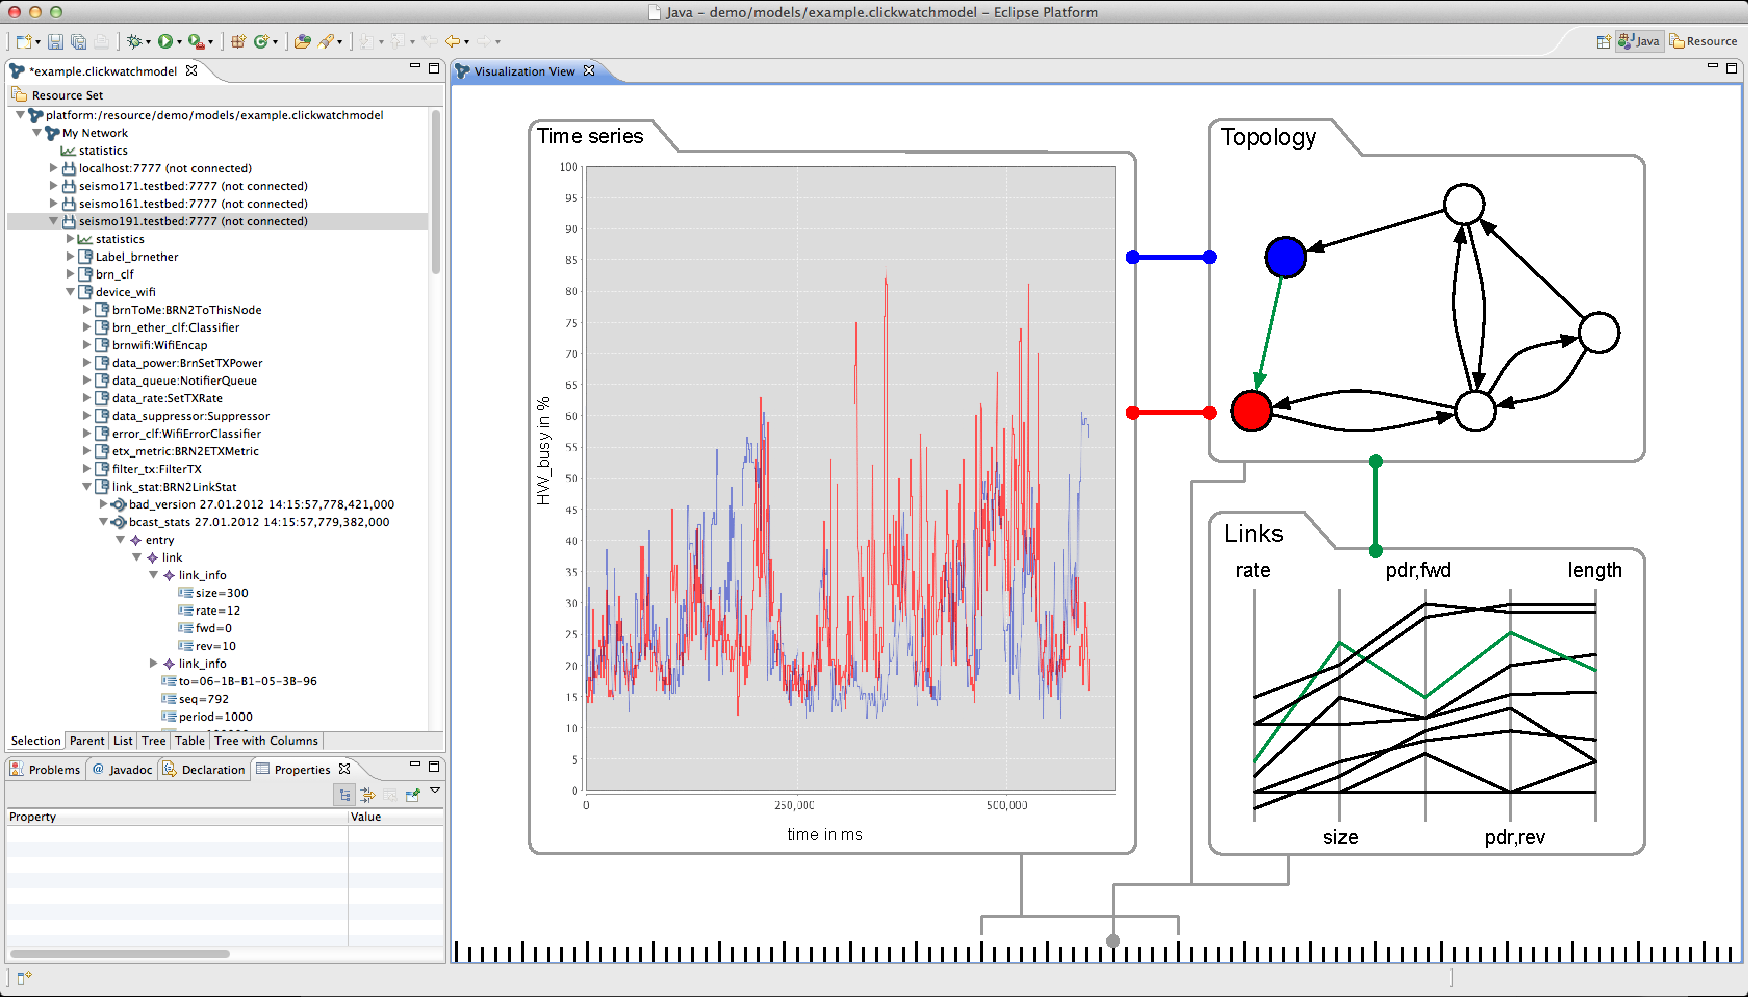
\includegraphics[width=\linewidth]{figures/final_goal_mockup}
  \caption{A mock-up screen shot of a tool that visualizes relations in different analysis results.}
  \label{fig:final_goal_mockup}
\end{figure}

Fig.~\ref{fig:final_goal_mockup} shows a mock-up of an screen shot of an potential data analysis visualization.
The screen shows the results of different analysis threads of the same WSN: the topology, properties of links, time series on the busyness of the radio hardware, and a time reference. 
The different results are related to each other. The link properties are related to the links in the topology; the time series are related to the nodes are taken from; and each result is related to a point or frame in time.

\subsection{The Problems}

\paragraph{Problem 1: No Traces on Model-Level}
Data analysis takes an initial set of data and produces new sets of data in a sequence of analysis steps. During this process no traces between the different data items are created. This means there is no formal relationship between elements on the data-level (model-level). Formal relations do only exist on the analysis-level (meta-model-level). These relations are defined by the analysis description. 

\paragraph{Problem 2: No Feasible Data Store for Related Analysis Results}
If we would keep traces between analysis results, initial data, analysis results and traces would form one interconnected information model (graph, refer. to Fig.~\ref{fig:example_analysis_data}. This information model must be accessed (navigation along traces) efficiently. 

\paragraph{Problem 3: Relations on Model-Level can only Be Seen In Context Of Relations on Analysis-Level}
Imagine an example drawn from a WSN analysis. The analysis has three threads and therefore produces three results for each node. We take a single result from one thread and are interested in the related result of another thread. We can navigate the trace of the taken result back to its origin. When we reach the origin, we are confronted with a multitude of different traces and we can only determine their meaning if we look at the analysis description. We need to know two things, which traces correspond the the second tread we are interested in, and which traces belong to the node that our original value belonged to. The analysis descriptions can tell us, how each trace was produces. Hence, if we look on the relations on both model and analysis-level, we can answer the questions.

\paragraph{Problem 4: Implicit Relations in the Initial Data}
Items in the initial data often contains string references to other data items. These references represent links that are valuable to the analysis and to our efforts to relate analysis results to each other. In order to use them, these implicit links need to be made explicit. String references must be resolved and replaces by actual model links.
 
\subsection{The Solution}

\paragraph{Solution to Problem 1: Model-Level Traces}
Typical ways to describe data analysis is using languages such as Matlab, R, Java. We can't change that. Therefore, we need a language that allows us to describe analysis as before, but in its semantics does not only realise the analysis but also creates traces and annotates the result accordingly. 

Language like Scala provide enough flexibility to provide internal languages that might look like regular programming/analysis/transformation languages, but also hide additional behaviour. We will use Scala to provide an analysis language that creates traces transparently. 

\paragraph{Solution to Problem 2: Data Store}
Large (EMF) models can be stored to different resources. The model is fragmented into different fragments and each fragment is stored in its own resources. References between fragments are realized with URIs identifying elements in different resources. 

We use a key-value data store (e.g. HBase) to store large models. Each resource becomes a value and the resource URI the key. With clever fragmentation the model can be created and accessed fast. For example, to navigate a $n$-depth analysis thread to a related item in another thread, in a model with $m$ data items, it always takes less then $2\left(\mathcal{O}n*log(m)\right($ to access the origin and navigate to the related data item of another thread.

\paragraph{Solution to Problem 3: Model-Level and Analysis-Level Relations}
\markus{Is this really a problem?}

\paragraph{Solution to Problem 4: Implicit References} 
There are obvious solutions, but we need on that operates of automatically as possible. One approach is to annotate the meta-model (which is generated in case of ClickWatch and HWL). 


\input{analysis_traces}

\section{Storing Large Models (Problem 2)}
Please refer to the paper \emph{Model Fragmentation For High Access Performance of Models Persisted in Key-Value Stores}.


\bibliography{bibliography}

\end{document}
